\documentclass[aspectratio=169,t]{beamer}
\usepackage{slides}
\title{The Urban Wage Premium in Historical Perspective}
\date{\today}
\author{Kyle Butts, Taylor Jaworski, and Carl Kitchens}
\addbibresource{urban_wage_biblio.bib}

\newcommand{\urban}{{\text{Urban}}}

\begin{document}

% ------------------------------------------------------------------------------
\begin{frame}
\maketitle

% \vspace{2.5mm}
% {\footnotesize $^*$ A bit of extra info here. Add an asterich to title or author}
\end{frame}
% ------------------------------------------------------------------------------

\section*{Motivation}

\begin{frame}{}
  \begin{center}
    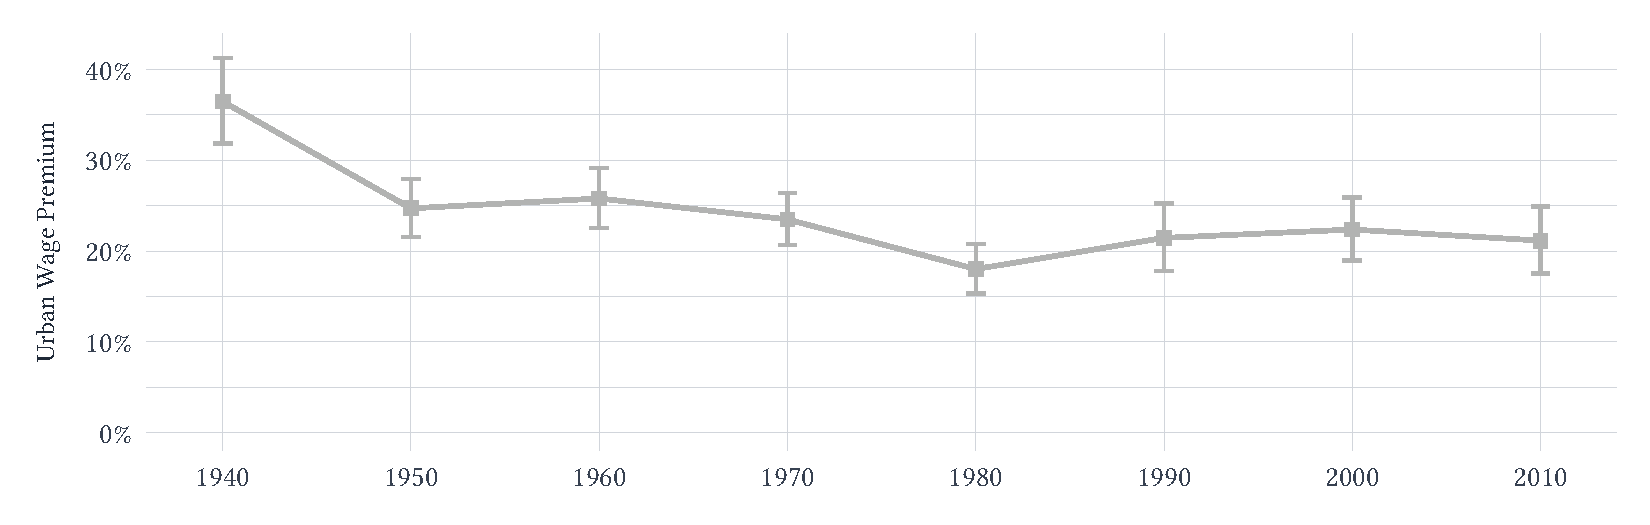
\includegraphics[width = \textwidth]{figures/slides/raw_premium.pdf}
  \end{center}

  \bigskip
  In the U.S. today, workers that live in an urban area earn $\approx$ 22\% more than non-urban workers
  \begin{itemize}
    \item This pattern holds in cities across the world and over (at least) the last 80 years in the US \citep{Boustan_Bunten_Hearey_2013}
  \end{itemize}
\end{frame}

\begin{frame}{Self-selection and the premium}
  While the raw data shows a large difference in earnings, it is not clear if this is a causal effect or due to non-random sorting
  \begin{itemize}
    \item College-educated and high-skilled workers are increasingly migrating to cities 
    
    {\small \citep{glaeser2001consumer,Combes_Duranton_Gobillon_2008,Diamond_2016,autorWorkPastFuture}}
  \end{itemize}

  \medskip\bigskip
  Indeed, panel data estimates shows the current causal wage premium is much smaller 
  \begin{itemize}
    \item \citet{Glaeser_Mare_2001} estimate effects between 5 to 10\% 

    \item For blue-collar workers, \citet{gould2007cities} estimate a wage premium of only 1.2 percent
  \end{itemize}
\end{frame}

\begin{frame}{Why study the historical urban wage premium?}
  Over time the economic structure of a city has changed 
  \begin{itemize}
    \item In the 1940s, cities were primarily manufacturing-based
    
    \item Moving towards service-sector in the 21st century \citep{Diamond_2016}
  \end{itemize}

  \bigskip
  Understanding the wage premium over the 20th century provides insights into how the benefits of urbanity changes over a country's development
  \pause
  \begin{itemize}
    \item Understanding the productivity benefits of cities in manufacture-based economies has strong implications for growth policies in developing countries
  \end{itemize}
\end{frame}

\begin{frame}{Past approach to estimating causal wage premium}
  The current literature focuses on a `movers' approach to estimating the causal wage premium. 
  Comparing individuals who enter or exit an urban location allows to control for `worker fundamentals'
  \begin{itemize}
    \item Individual level panel surveys begin after 1980

    \item Estimates consistently around 5 percent, 
    {\small e.g. \citet{Glaeser_Mare_2001}, \citet{Yankow_2006}, and \citet{BaumSnow_Pavan_2012}}
  \end{itemize}

  \bigskip
  More recent literature has tried to figure out determinents of the wage premium,
  \begin{itemize}
    \item {\small e.g. \citet{DCosta_Overman_2014}, \citet{card2024location}, and \citet{ananat2018race}}
  \end{itemize}
\end{frame}

\begin{frame}{Studying the historical urban wage premium is hard}
  Without panel data, the standard approach is infeasible for estimating a historical causal wage premium

  \bigskip
  We use the approach of \citet{altonji2018estimating} to estimate causal urban-wage premium in cross-sectional census data
  \begin{itemize}
    \item Leverage properties of the canonical location-choice model to control for differences in average unobservables between urban and non-urban locations
  \end{itemize}
\end{frame}

% \begin{frame}{Preview of Results}
% TODO:
% \end{frame}

\section{Data and Empirical Strategy}

\begin{frame}{Data Sources}
  We use various U.S. Census surveys for each decade from 1940 to 2010:
  \begin{itemize}
    \item 1940: complete count census
    
    \item 1960--1970: 5\% census samples
    
    \item 1950, 1980, 1990, and 2000: 1\% census sample
    
    \item 2010: American Community Survey
  \end{itemize}
  
  \bigskip
  We restrict the sample to
  \begin{itemize}
    \item adult males between ages 25 and 65,
    \item and report being employed for at least 26 weeks in the year
  \end{itemize} 
\end{frame}

\begin{frame}{Observable covariates}
  The main outcome variable is $\log$ weekly wage
  \begin{itemize}
    \item total annual earnings $/$ the number of weeks worked
  \end{itemize}

  \bigskip
  The census data provides limited consistently measured characteristics
  \begin{itemize}
    \item age, race, educational attainment, marital status, and veteran status
  \end{itemize}

  \pause
  \bigskip
  Later, we consider a measure of `real wage' premium that adjusts for housing costs. Following \citet{ganong2017has}, we form an individual measure of housing costs 
  \begin{itemize}
    \item 5\% of reported housing value or 12$\times$ reported monthly rent.  Divide by 48 to get the weekly housing costs
  \end{itemize}
\end{frame}

\begin{frame}{Definition of Urban Area}
  Our definition of `urban' is defined as the Metropolitan Statistical Areas
  \begin{itemize}
    \item MSAs cover urban core and suburbs where residents live
  \end{itemize}

  \bigskip
  For non-urban areas, we group together all counties not in an MSA by state
  \begin{itemize}
    \item 48 non-urban areas for people to live-in
  \end{itemize}
\end{frame}

% \begin{frame}{Definition of Urban Area}
%   \vspace*{-2\bigskipamount}
%   \begin{center}
%     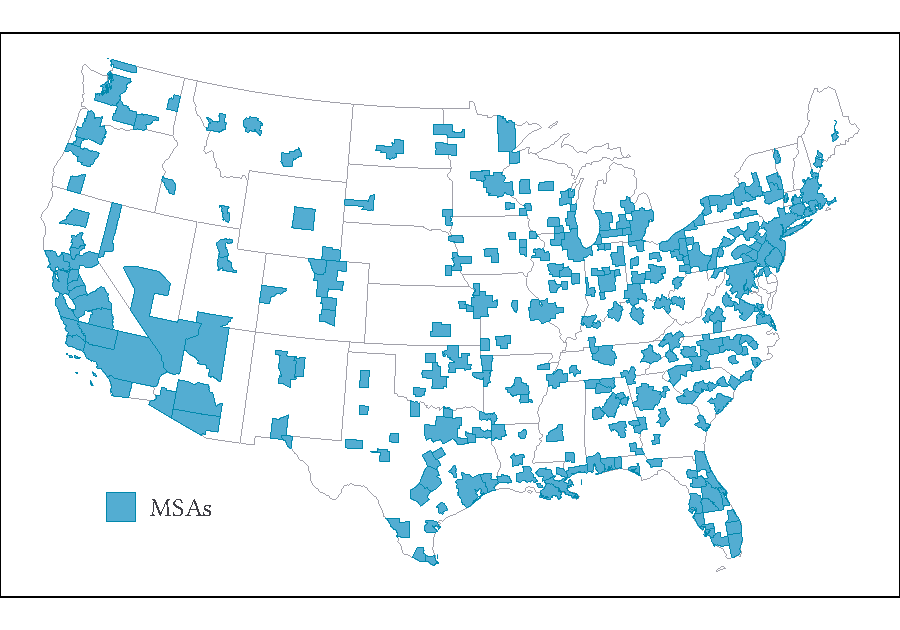
\includegraphics[width=0.75\textwidth]{figures/slides/map_msa.pdf}
%   \end{center}
% \end{frame}

\imageframe{figures/slides/map_msa.pdf}

% \begin{frame}{}
%   \centering
%   \begin{tabular}{@{} c @{\extracolsep{20pt}} c @{\extracolsep{5pt}} cccc @{}}
%     % Head
%     \toprule
% 
%     & & & \multicolumn{3}{c}{\% With College Degree} \\
%     \cmidrule{4-6}
%     Year & \multicolumn{1}{c}{\% Wage Gap} & \multicolumn{1}{c}{\% Urban} & \multicolumn{1}{c}{Overall} & \multicolumn{1}{c}{in Urban} & \multicolumn{1}{c}{in Non-urban} \\
%     (1) & \multicolumn{1}{c}{(2)} & \multicolumn{1}{c}{(3)} & \multicolumn{1}{c}{(4)} & \multicolumn{1}{c}{(5)} & \multicolumn{1}{c}{(6)} \\  
% 
%     % Body
%     \toprule
% 
%     1940 & 31.4 & 65.6 & 8.4 & 8.8 & 7.6 \\
1950 & 21.6 & 68.3 & 8.0 & 8.6 & 6.7 \\
1960 & 23.5 & 65.2 & 11.5 & 12.9 & 9.1 \\
1970 & 23.5 & 74.4 & 16.6 & 17.8 & 13.0 \\
1980 & 19.3 & 72.2 & 24.1 & 26.6 & 17.7 \\
1990 & 25.7 & 73.2 & 28.0 & 31.1 & 19.6 \\
2000 & 31.6 & 78.4 & 30.5 & 33.4 & 19.8 \\
2010 & 30.2 & 79.1 & 33.5 & 36.4 & 22.2 \\

% 
%     \bottomrule
%   \end{tabular}
% \end{frame}

\begin{frame}{Empirical Strategy}
  We consider the following regression specifications:
  $$
    \log(\text{wage}_i) = \beta_0 + \beta_1 \urban_i + \bm{W}_i \delta + u_i
  $$
  Regressions are run separately by year and $\hat{\beta}_1$ is our wage-premium estimate for that year

  \begin{itemize}
    \item $\bm{W}_i$ are a set of worker characteristics that vary across specification
  \end{itemize}
\end{frame}

\begin{frame}{Individual level Controls}
  Without covariates, the raw premium (no covariates) is what we presented on the first slide 

  \bigskip
  As a first pass, we control for a set of individual characteristics
  \begin{itemize}
    \item 5-year age bins
    \item Years of schooling
    \item indicator for being White
  \end{itemize}
\end{frame}

\begin{frame}[plain]{Controlling for Individual-level Characteristics}
  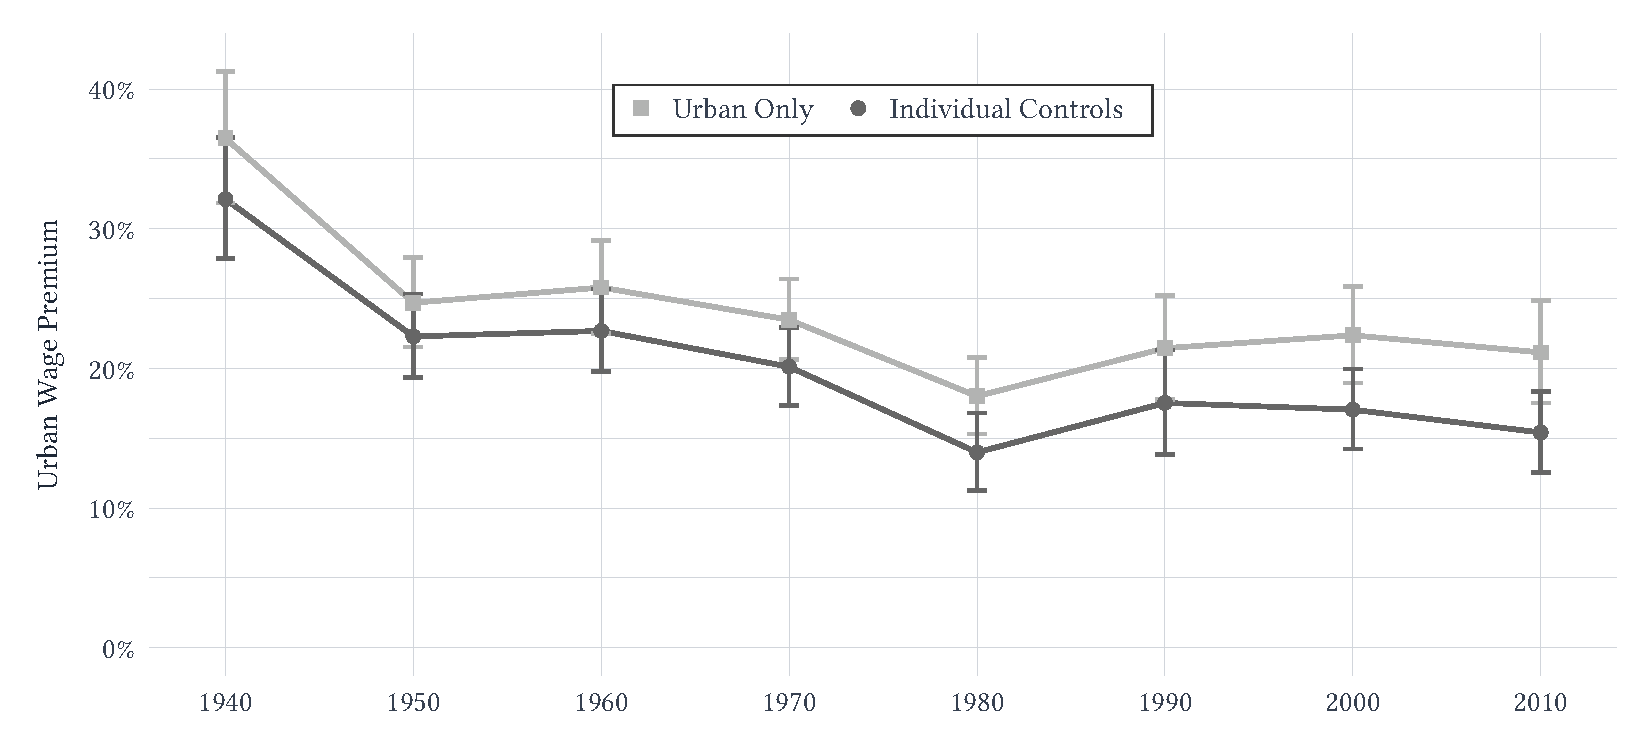
\includegraphics[width=\textwidth]{figures/urban_premium/controls.pdf}
\end{frame}

\begin{frame}{Individual level Controls}
  \textbf{Takeaway:} The individual controls absorb a small portion of the raw premium
  \begin{itemize}
    \item Much less explained than suggested by the standard ``urban-living college worker'' story
  \end{itemize}

  \bigskip
  The estimates in later periods are much larger compared to panel data estimates
\end{frame}


\section{Causal Wage Premium}

\begin{frame}{Controlling for Unobservables}
  In this section, we lay out the methodology to estimate the causal urban wage premium in our cross-sectional setting
  \begin{itemize}
    \item Follow closely to \citet{altonji2018estimating}
  \end{itemize}
\end{frame}

\begin{frame}{Omitted Variables Bias}
  \vspace{-\bigskipamount}
  $$
    \log(\text{wage}_i) = \beta_0 + \beta_1 \urban_i + \bm{W}_i \delta + u_i
  $$

  For intuition, think about the bias of $\hat{\beta}_1$: 
  \begin{itemize}
    \item Biased by differences in average of unobservables for urban compared to non-urban areas (multiplied by their marginal effect)
  \end{itemize}

  \pause
  \bigskip
  \hspace{1ex}$\implies$ It would be sufficient to control for location-specific $\bar{\bm{Z}}_{\ell(i)}$, though these are unobservable
\end{frame}

\begin{frame}{Identification example}
  Think of a single unobservable characteristic: \emph{curiosity}

  \bigskip
  More curious workers might prefer to live in urban locations that offer more consumptive amenities (e.g. \emph{live entertainment} or \emph{more food options})
  \begin{itemize}
    \item Biases our urban wage premium estimate
  \end{itemize}
\end{frame}

\begin{frame}{Identification example}
  However, workers may sort based on age for these very same consumptive amenities.
  The amenities will `link' observable and unobservable characteristics:

  \begin{center}\large
    Curiosity $\leftrightarrow$ Live Entertainment $\leftrightarrow$ Age
  \end{center}

  \bigskip
  Allows us to correct for differences in unobservables between urban and non-urban workers. 
\end{frame}

\begin{frame}{Location-choice model}
  The canonical location-choice model has worker $i$ choosing over locations, $\ell$, to maximize their indirect utility 
  \vspace*{-\bigskipamount}
  $$
    V_{i \ell} = \bm{W}_i \bm{A}_\ell - {P}_\ell + \varepsilon_{i \ell} 
  $$
  
  \vspace*{-\medskipamount}
  \begin{itemize}
    \item $\bm{A}_\ell$ is a vector of location-specific amenities
    \item $P_\ell$ is the housing costs in location $\ell$
    \item $\varepsilon_{i \ell}$ are idiosyncratic preference draws (assumed Type-1 EV)
  \end{itemize}

  \bigskip
  To allow for rich sorting patterns, the willingness to pay for amenities varies by worker, $\bm{W}_i$
  \begin{itemize}
    \item E.g. college workers have preferences for certain consumptive amenities \citep{Diamond_2016}
  \end{itemize}
\end{frame}

\begin{frame}{Sorting by Characteristics}
  Since locations vary by their amenities $\bm{A}_\ell$, the kinds of individuals they attract will vary too
  
  \begin{itemize}
    \item In equilibrium, the location-average of observable characteristics are a function of the location's amenities $\bar{\bm{X}}_\ell = f(\bm{A}_\ell)$
  \end{itemize}

  \pause
  \bigskip\medskip
  While we can not observe them, the location-average of \emph{unobservable characteristics} are also functions of amenities $\bar{\bm{X}}^U_\ell = f^U(\bm{A}_\ell)$
  \begin{itemize}
    \item The mapping and even which amenities impact sorting can differ for observable and unobservable characteristics.
  \end{itemize}
\end{frame}

\begin{frame}{Inverting the relationship}
  \vspace*{-1.5\bigskipamount}
  $$
    \bar{\bm{X}}_\ell = f(\bm{A}_\ell) \ \text{ and }\  \bar{\bm{X}}^U_\ell = f^U(\bm{A}_\ell)
  $$

  \medskip
  Say we knew the mappings$f$ and $f^U$. Under conditions we will list below, we can `invert' observable averages to learn about amenities
  $$
    \bm{A}_\ell = f^{-1}(\bar{\bm{X}}_\ell)
  $$

  \pause
  \bigskip
  Then apply $f^U$ to learn about unobservables
  $$
    \bar{\bm{X}}^U_\ell = f^U(f^{-1}(\bar{\bm{X}}_\ell))
  $$
\end{frame}

\begin{frame}{Inverting the relationship}
  \vspace*{-1.5\bigskipamount}
  $$
    \bar{\bm{X}}^U_\ell = f^U(f^{-1}(\bar{\bm{X}}_\ell))
  $$

  \medskip
  Under the location choice and a set of assumptions, the location choice model implies that $f^U(f^{-1}(\cdot))$ is actually a \emph{linear mapping}, 
  $$\bar{\bm{X}}^U_\ell = \bar{\bm{X}}_\ell \Pi$$

  \pause
  \bigskip
  \textbf{\blue{Upshot}}: Controlling \emph{linearly} for $\bar{\bm{X}}_\ell$ in our wage premium model is sufficient to control for differences in unobservables between urban and non-urban locations
\end{frame}

\begin{frame}{Necessary Assumptions}
  The first three assumptions are standard:

  \begin{itemize}
    \item[\color{blue} A1] The indirect utility function is $V_{i \ell} = \bm{W}_i \bm{A}_\ell - {P}_\ell + \varepsilon_{i \ell}$
    
    \medskip
    \item[\color{blue} A2] $\varepsilon_{i \ell}$ are iid type-1 Extreme Value 
    \begin{itemize}
      \item standard in urban/trade literature
    \end{itemize}
    
    \medskip
    \item[\color{blue} A3] When choosing locations, workers take prices and amenities as given 
    \begin{itemize}
      \item They do not internalize their own effect on prices and amenities
    \end{itemize}
  \end{itemize}
\end{frame}


\begin{frame}{Necessary Assumptions}
  The next two assumptions restrict the relationship between observables, unobservables, and amenities. Remember our mapping relies on:

  \bigskip
  Observables teach us about amenities
  \begin{itemize}
    \item[\color{blue} A4] The function $A_\ell = f(\bar{X}_{\ell})$ is invertible
    \begin{itemize}
      \item For each amenity, we need some $X_i$ that explains differences in WTP for that amenity
    \end{itemize}
  \end{itemize}

  \pause
  \bigskip
  Amenities teach us about unobservables
  \begin{itemize}
    \item[\color{blue} A5] The set of location-specific amenities that drive sorting on observables contains all amenities that drive sorting based on unobservable covariates
  \end{itemize}
\end{frame}

\begin{frame}{Result from \citet{altonji2018estimating}}
  With assumptions {\color{blue} A1}-{\color{blue} A5}, the location choice model implies the mapping between $\bar{X}_{\ell}$ and $\bar{X}^U_{\ell}$ is linear
  
  \bigskip
  We leverage this to isolate the \emph{causal} urban wage premium by modifying our estimation equation to include a set of location-averages of observable characteristics
  $$
    \log(\text{wage}_i) = \beta_0 + \beta_1 \urban_i + \bm{W}_i \delta + \bar{\bm{X}}_\ell \gamma + u_i
  $$
\end{frame}

\begin{frame}{Group Averages}
  For our group-averages, we include variables we think explain differences in WTP for amenities:
  \begin{itemize}
    \item the share of white workers (the share of non-white workers drops out)
    \item share of residents in each 5-year age bin
    \item share of veterans
    \item share of married and together, married and apart, and single
    \item share with $<$ HS, HS degree, some college, BA degree, and post-secondary education
    \item a measure of market access calculated as in \citet{Jaworski_Kitchens_2019} 
  \end{itemize} 
\end{frame}

\begin{frame}{Plausibility of {\color{blue} A4}}
  While there are theoretically many amenities people can `shop with their feet for', many are tightly bundled together
  \begin{itemize}
    \item Using a principle components analysis on a wide array of amenities, \citet{Diamond_2016} finds 5 `bundles' of amenities across locations 
  \end{itemize}

  \bigskip
  Therefore, we need the effective rank of our group averages to be 5 or larger
  \begin{itemize}
    \item Running a similar PCA, we find 6 components explain more than 5 percent of the variance across years
  \end{itemize}
\end{frame}

\begin{frame}{Plausibility of {\color{blue} A5}}
  
  {\color{blue} A5} is a more difficult assumption to assess since it is an assumption about unobservable characteristics
  \begin{itemize}
    \item Later, we think our ability to match estimates in 2000 and 2010 help alleviate concerns about failing to control for unobservables 
  \end{itemize}
\end{frame}


\begin{frame}[plain]{Causal Urban Wage Premium Estimates}
  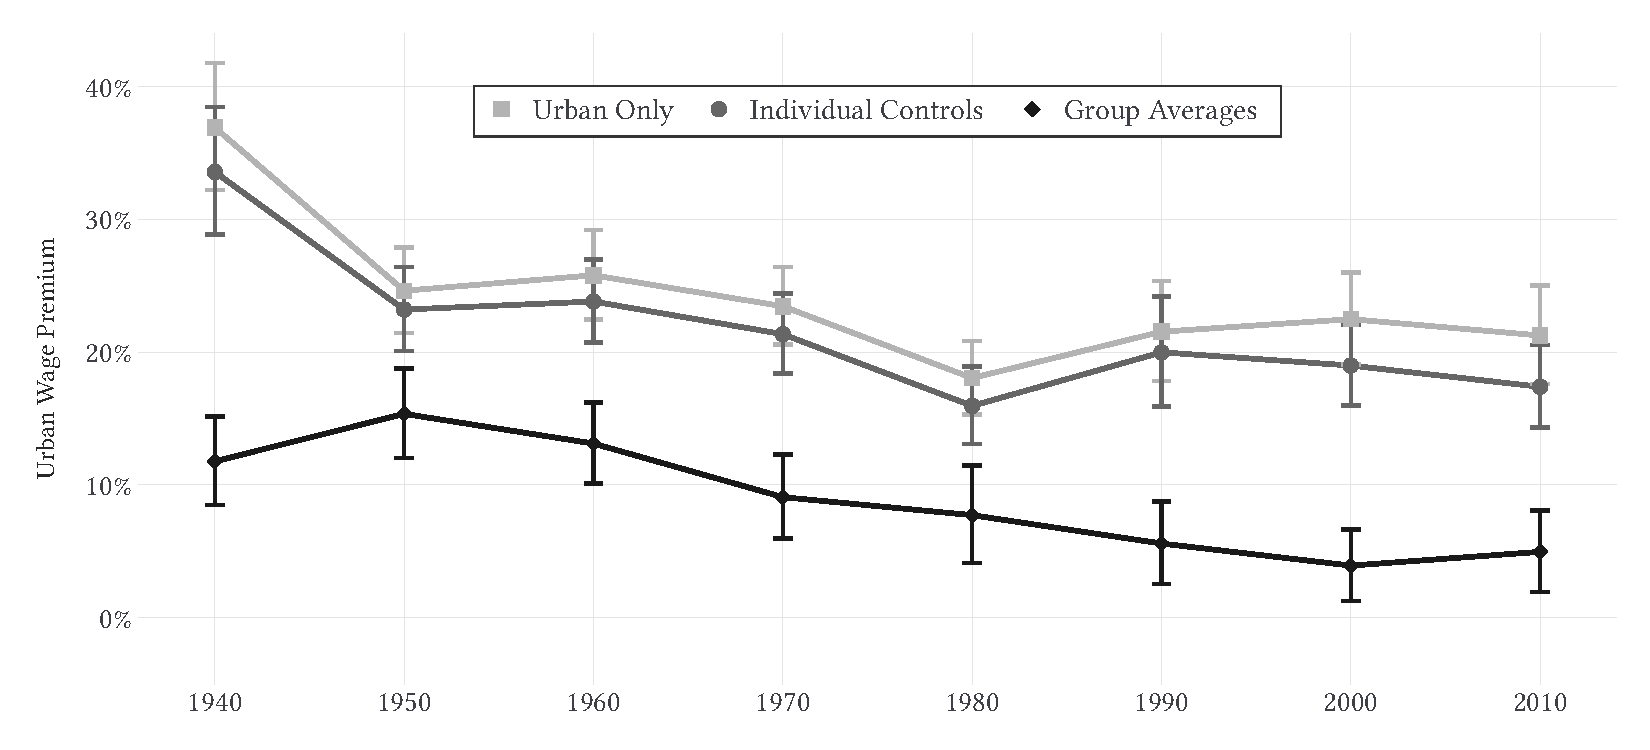
\includegraphics[width=\textwidth]{figures/urban_premium/combined.pdf}
\end{frame}


\begin{frame}{Takeaways}
  From 1990--2010, the causal premium estimate is around 5\%, in line with results from \citet{Glaeser_Mare_2001,gould2007cities}
  \begin{itemize}
    \item This gives us confidence in our ability to control for sorting based on unobservables
  \end{itemize}
  
  \pause
  \bigskip
  Looking into past decades, the causal estimates grow over time, peaking between 12 and 15\% in the middle of the 20th century
  
  \bigskip
  In line with the historical evidence:
  \begin{itemize}
    \item In middle 20th century, manufacturing bases in cities offering higher wages
    
    \item Decline in wage premium concurrent with sub-urbanization
  \end{itemize}
\end{frame}

\begin{frame}{Wages net of Housing Costs}
  Of course, urban areas also face higher housing costs
  \begin{itemize}
    \item Higher wages workers receive might be extracted by landlords via higher rent
  \end{itemize}

  \pause
  \bigskip
  We rerun our analysis using $ \log(\text{wage}_i - P_{\ell})$
  \begin{itemize}
    \item Following \citet{ganong2017has}, 5\% of reported housing value or 12$\times$ reported monthly rent. Divide by 48 to get the weekly housing costs
    \begin{itemize}
      \item Averaged over individuals to abstract from individual preferences for housing
      
      \item The 1950 census had no housing estimates, so we use an aggregate housing cost measure from the Census
    \end{itemize}
  \end{itemize}
\end{frame}

% \begin{frame}[plain]{Urban Housing Cost Premium}
%   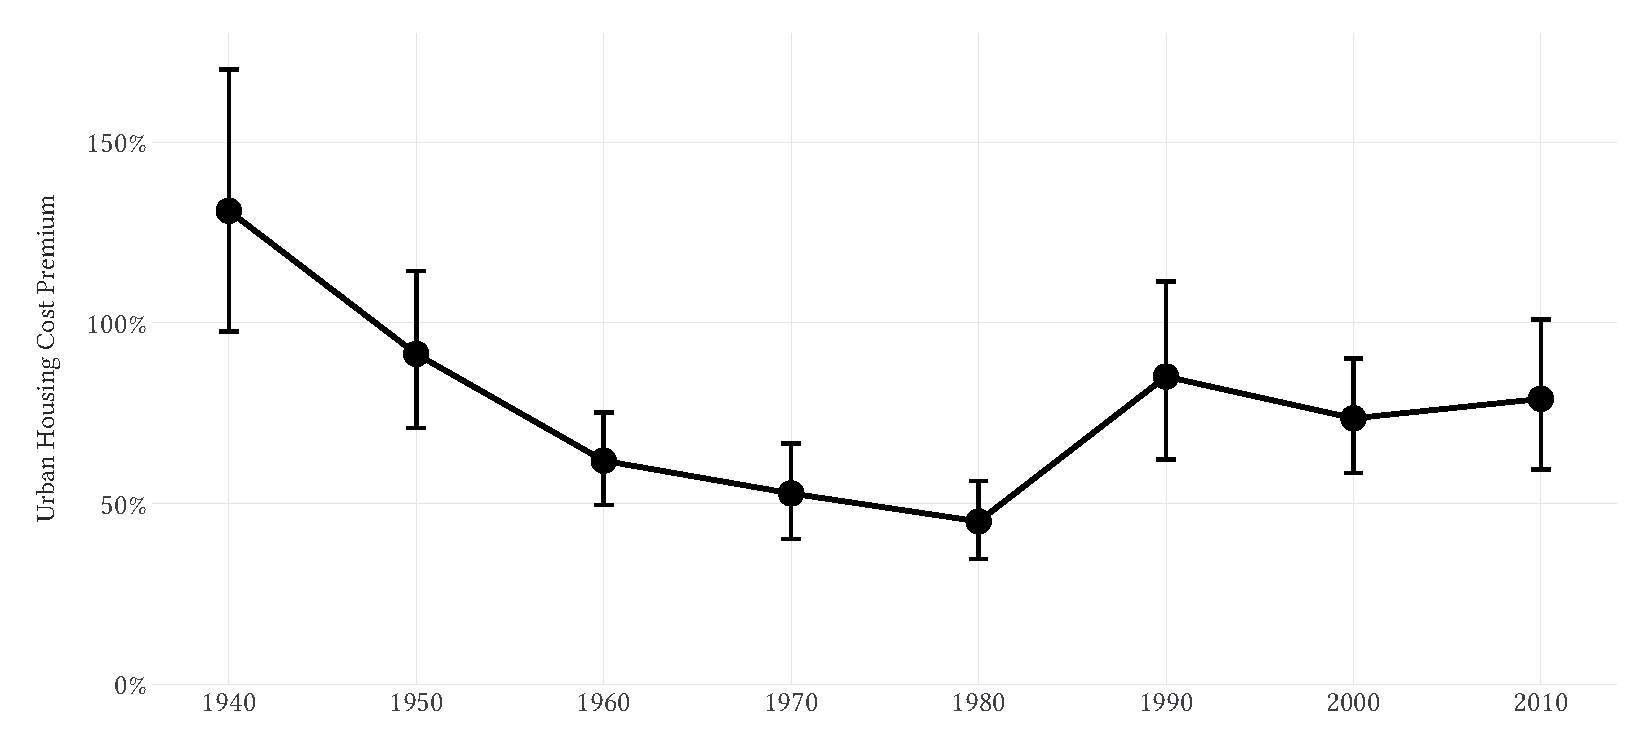
\includegraphics[width=\textwidth]{figures/housing_costs/raw_housing_costs_differences.pdf}
% \end{frame}

\begin{frame}[plain]{Raw Urban (Net of Housing) Wage Premium Estimates}
  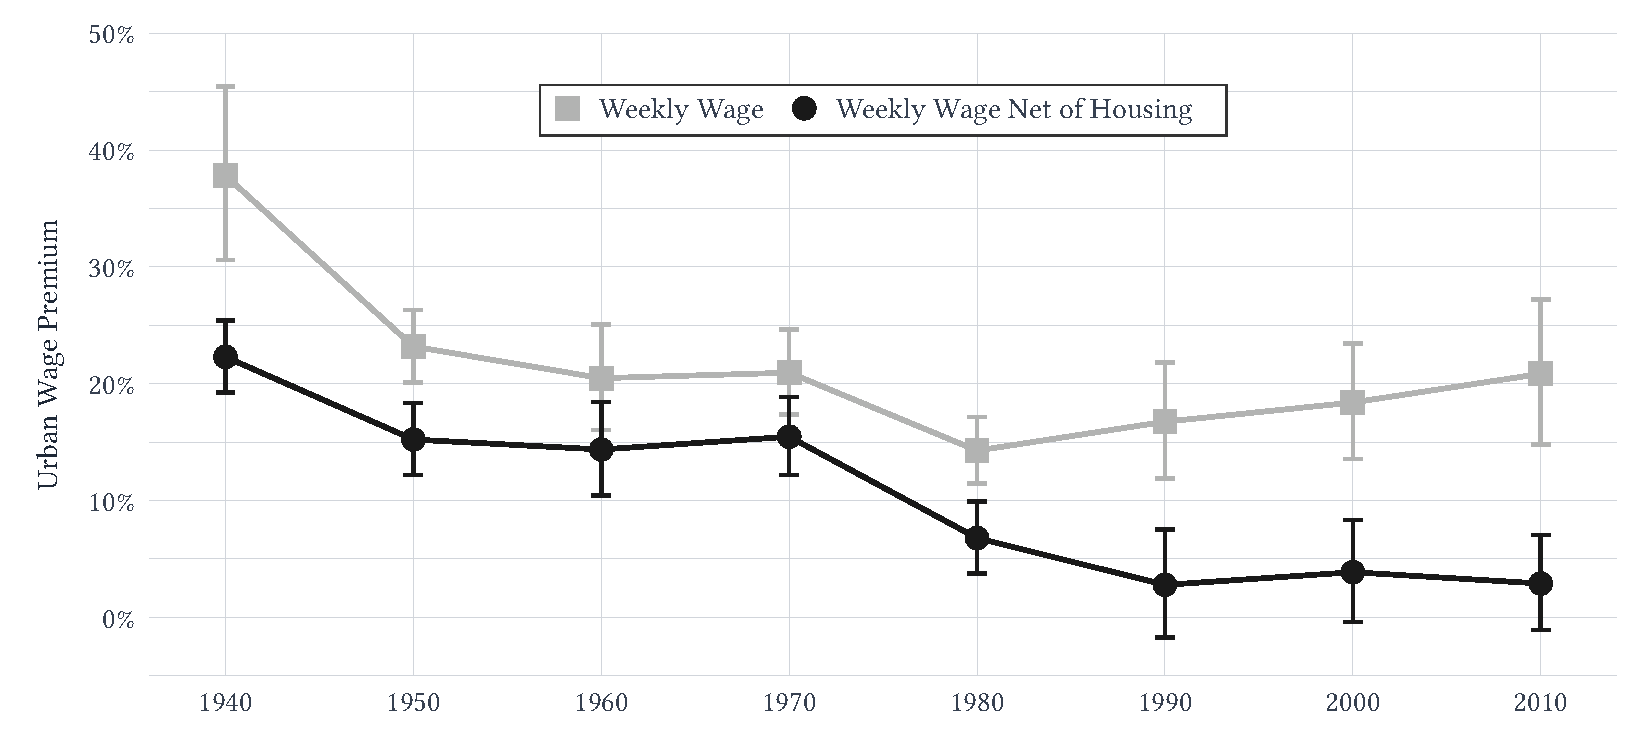
\includegraphics[width=\textwidth]{figures/housing_costs/net_raw.pdf}
\end{frame}

\begin{frame}[plain]{Causal Urban (Net of Housing) Wage Premium Estimates}
  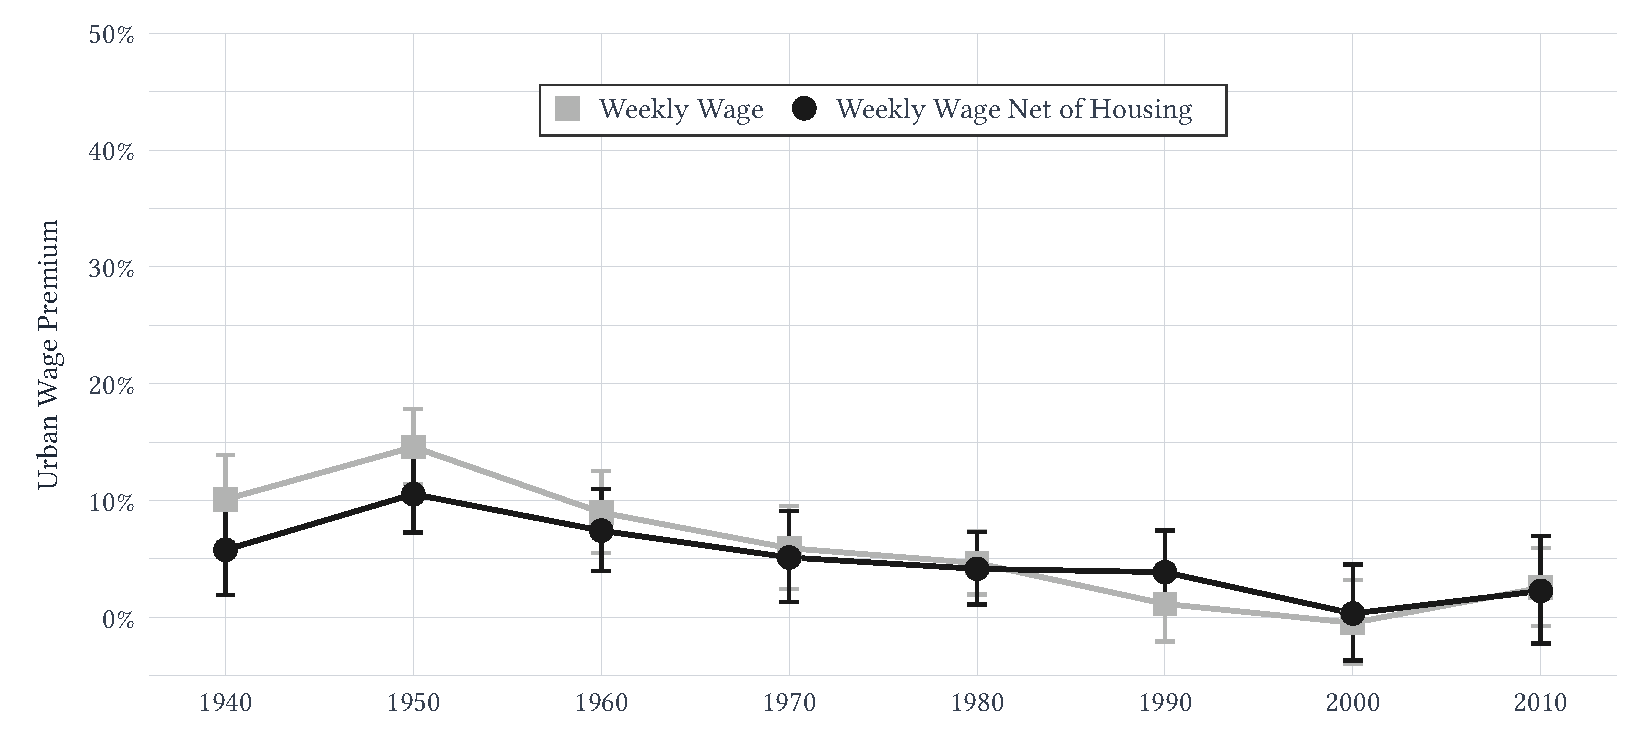
\includegraphics[width=\textwidth]{figures/housing_costs/net_causal.pdf}
\end{frame}


\section{Heterogeneity Results}

\begin{frame}{Heterogeneity by City Size}
  Next, we explored heterogeneity in the causal wage premium.

  \bigskip
  First, the literature has shown that larger cities have a larger causal premium \citep{BaumSnow_Pavan_2012,Glaeser_Mare_2001}
  \begin{itemize}
    \item We interact the urban indicator with being a large MSA ($\geq 1$ million population)
  \end{itemize}
\end{frame}

\begin{frame}[plain]{Heterogeneity by City Size}
  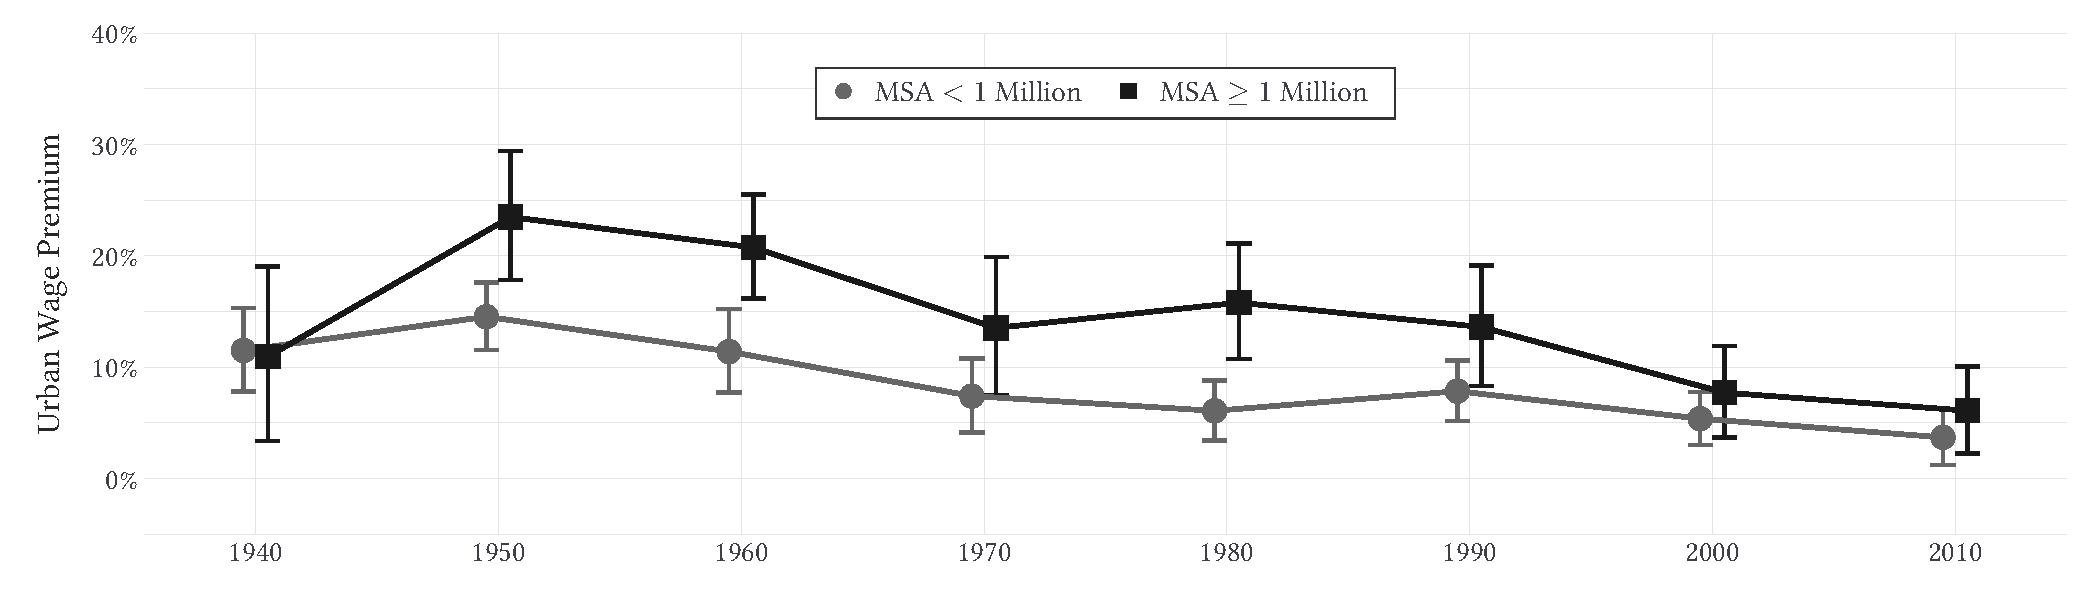
\includegraphics[width=\textwidth]{figures/heterogeneity/big_vs_small_cities.pdf}

  \bigskip
  Indeed we see the wage premium is moderately larger across years \citep{BaumSnow_Pavan_2012}, but the difference has shrunk in recent decades
  \begin{itemize}
    \item Consistent with the theory of sorting being increasingly important
  \end{itemize}
\end{frame}


\begin{frame}[plain]{Heterogeneity by Census Region}
  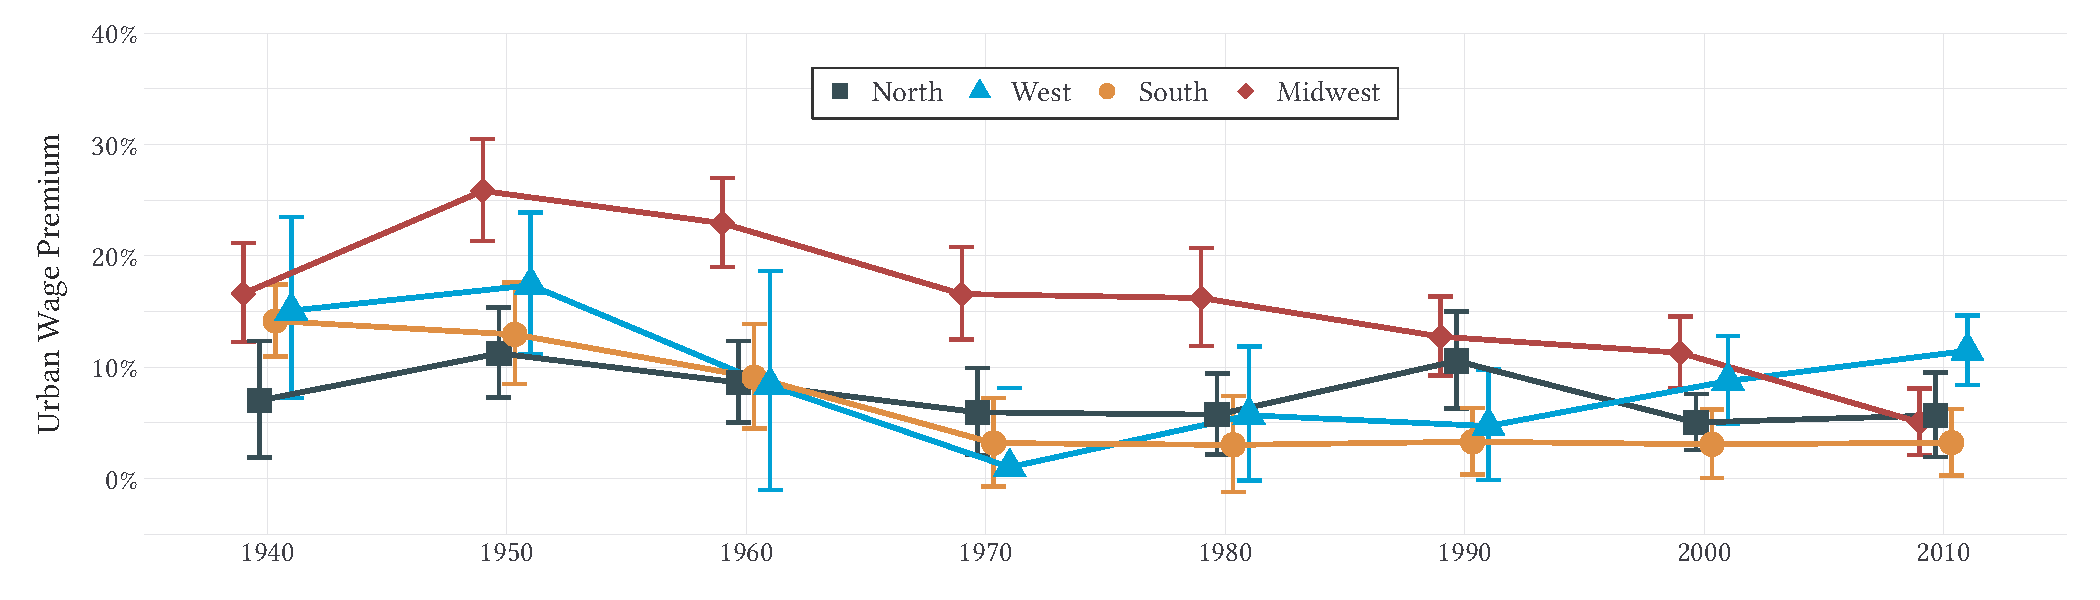
\includegraphics[width=\textwidth]{figures/heterogeneity/by_region.pdf}

  \begin{itemize}
    \item The Midwest had a much higher wage premium, consistent with cities' historical premium being driven by manufacturing
    \item A recent rise in the West's premium, consistent with technology sector
  \end{itemize}
\end{frame}

\begin{frame}[plain]{Heterogeneity by Manufacturing Sector}
  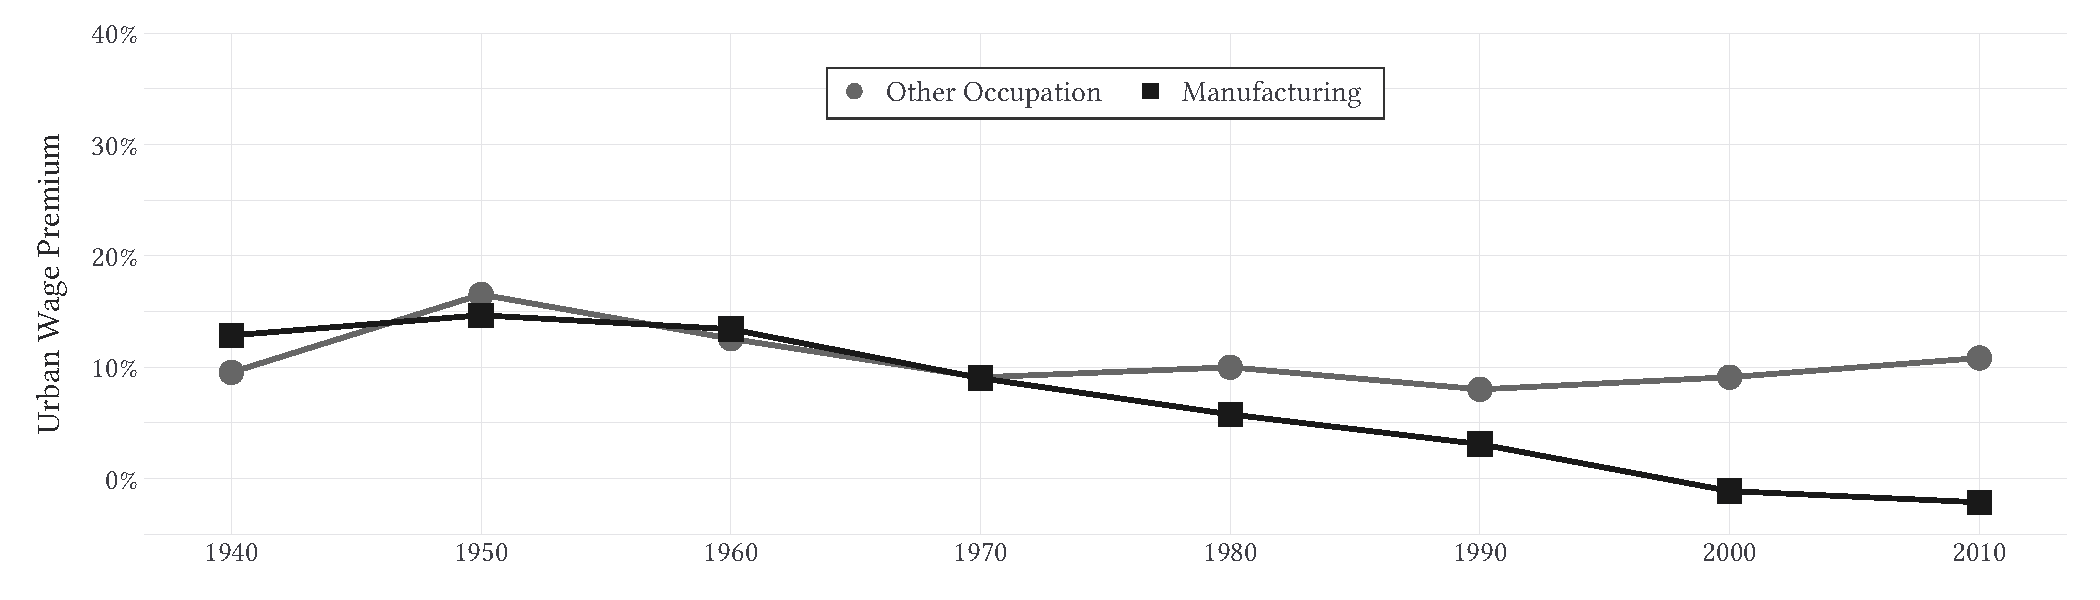
\includegraphics[width=\textwidth]{figures/heterogeneity/by_manufacturing.pdf}

  \begin{itemize}
    \item 
  \end{itemize}
\end{frame}



\begin{frame}{Heterogeneity for groups of workers}
  Next, we present three forms of worker-heterogeneity: college education and race
  \begin{itemize}
    \item For each, we take include separate group-averages by race/education because the sorting patterns (and hence linear mappings) might differ by these categories
  \end{itemize}
\end{frame}

\begin{frame}[plain]{Heterogeneity by College Education}
  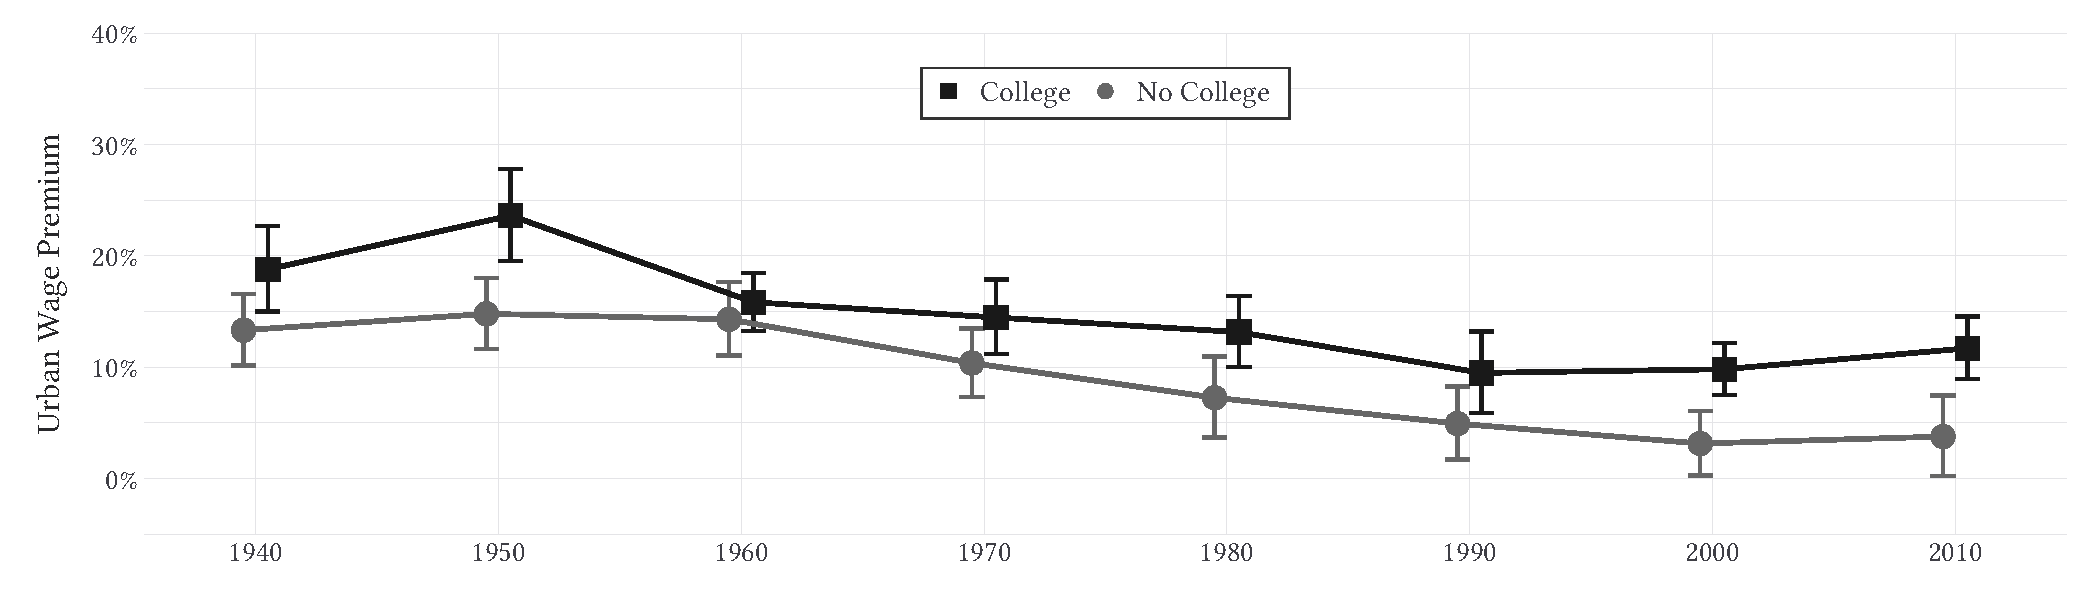
\includegraphics[width=\textwidth]{figures/heterogeneity/by_college.pdf}

  \bigskip
  The wage-premium is smaller for non-college educated workers, consistent with \citet{gould2007cities} and \citet{carlsen2016education}
\end{frame}

\begin{frame}[plain]{Heterogeneity by Race}
  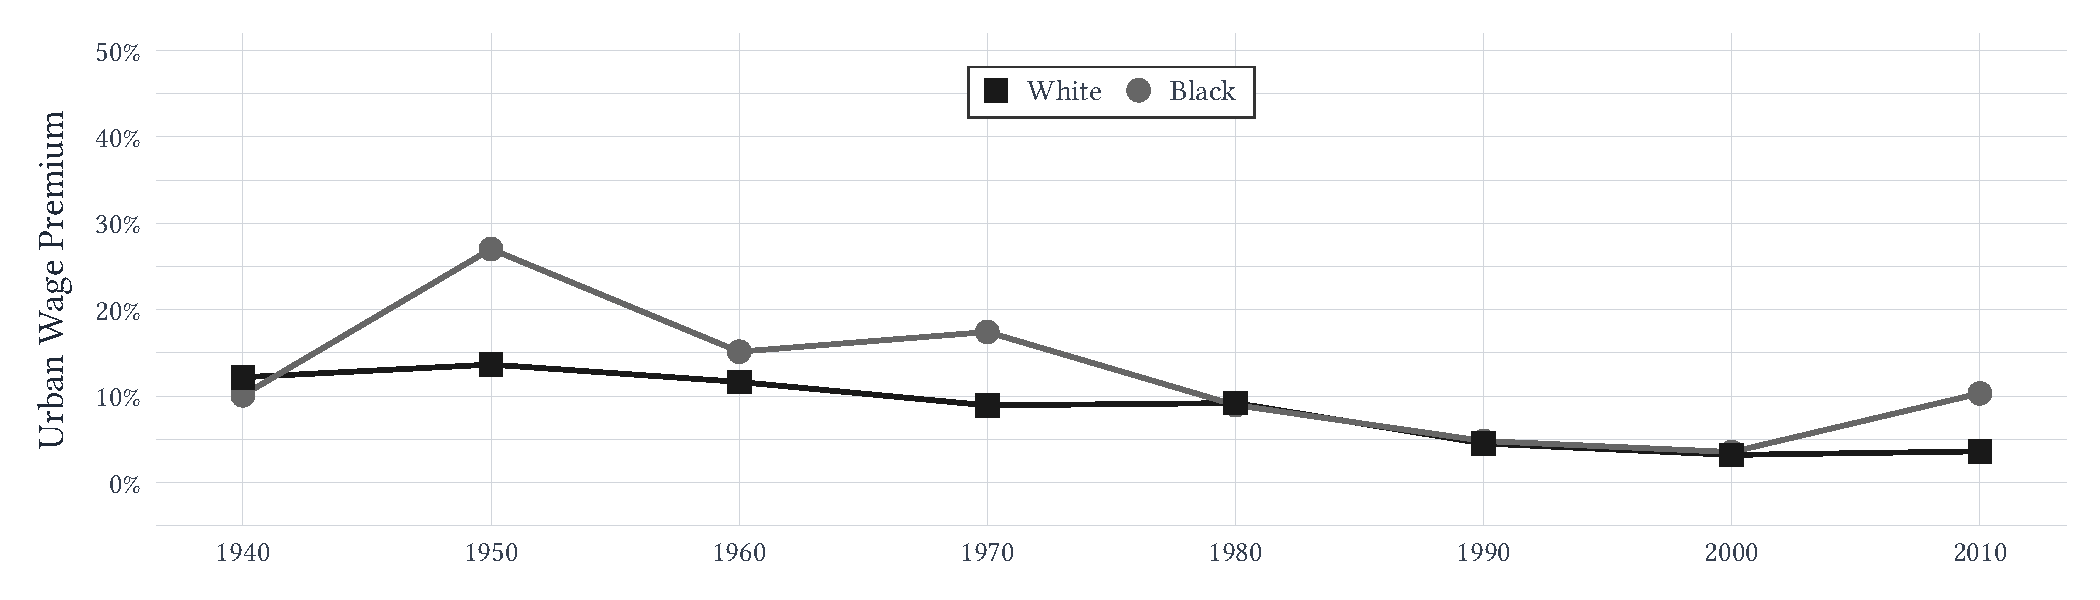
\includegraphics[width=\textwidth]{figures/heterogeneity/by_race.pdf}

  \bigskip
  The relatively higher wage premium by Black workers occurs during the period of the Great Migration \citep{boustan2016competition}
\end{frame}

\begin{frame}[plain]{Regional Heterogeneity for Black Workers}
  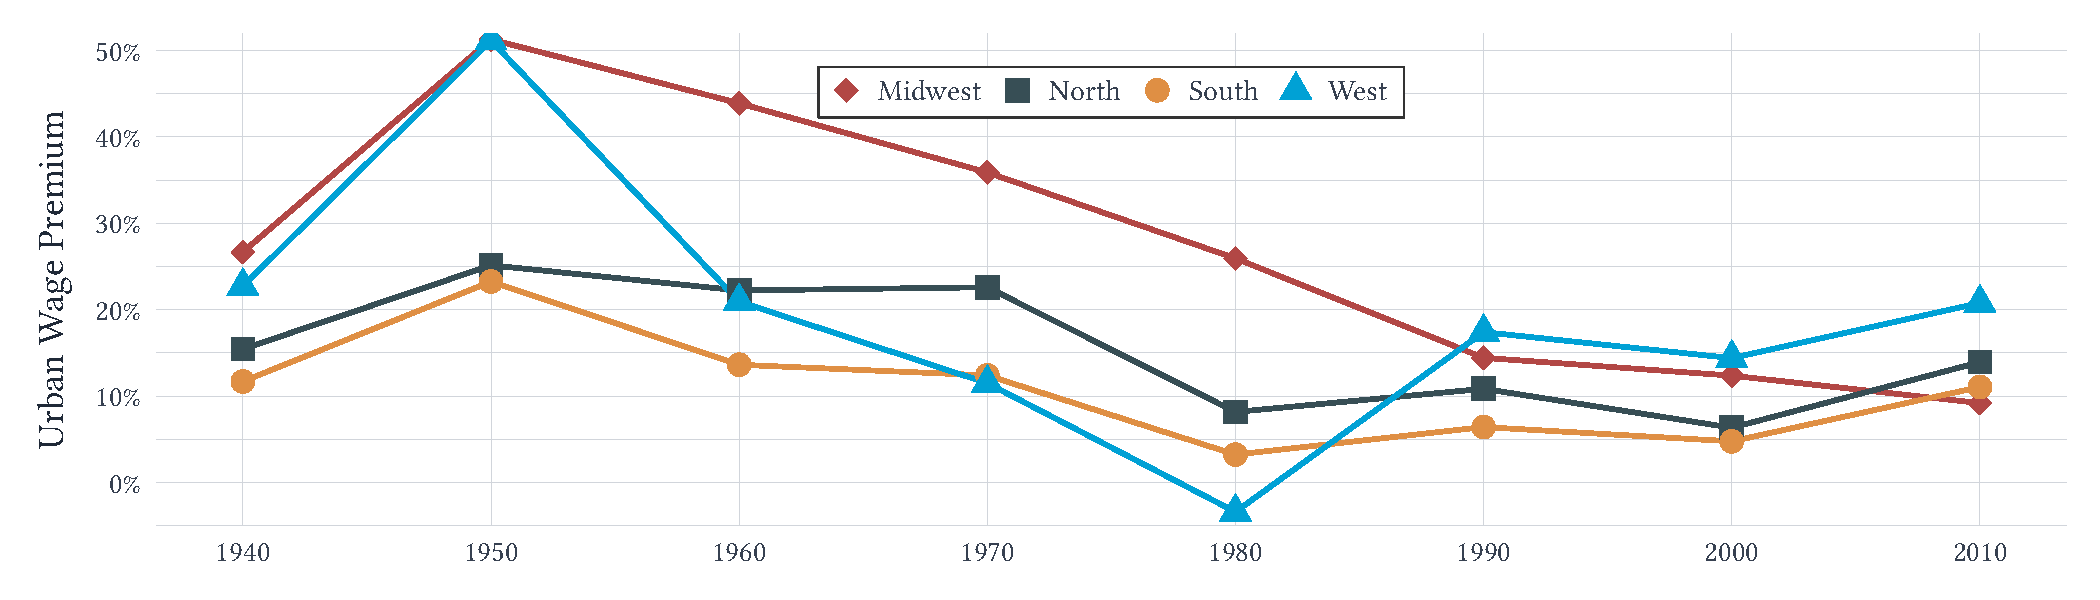
\includegraphics[width=\textwidth]{figures/heterogeneity/by_region_black.pdf}

  \bigskip
  At risk of stretching the data too thin, can see the Midwest and Western premiums served as a `pull factor' for the Great Migration
\end{frame}


\begin{frame}{Conclusion}
  Estimate a causal urban wage premium from 2010 back until 1940
  \begin{itemize}
    \item The causal premium was between 12 and 15\% in 1940--1960 and has shrunk over time to around 5\%
  \end{itemize}

  \bigskip
  Heterogeneity analysis in line with historical narrative:
  \begin{itemize}
    \item High-manufacturing in the Midwest gave high wage premia, particularly for Black workers
    
    \item College-educated workers benefit more from urbanity
  \end{itemize}

  \bigskip
  These result help us understand how agglomeration benefits accrue to workers at different points in economic development 
\end{frame}






% ------------------------------------------------------------------------------
\begin{frame}[allowframebreaks]{References}
  \printbibliography
\end{frame}
\appendix
% ------------------------------------------------------------------------------


\end{document}
